%
%   This file is part of the APS files in the REVTeX 4 distribution.
%   Version 4.0 of REVTeX, August 2001
%
%   Copyright (c) 2001 The American Physical Society.
%
%   See the REVTeX 4 README file for restrictions and more information.
%
% TeX'ing this file requires that you have AMS-LaTeX 2.0 installed
% as well as the rest of the prerequisites for REVTeX 4.0
%
% See the REVTeX 4 README file
% It also requires running BibTeX. The commands are as follows:
%
%  1)  latex apssamp.tex
%  2)  bibtex apssamp
%  3)  latex apssamp.tex
%  4)  latex apssamp.tex
%
%\documentclass[prb,aps,nobibnotes,twocolumn,doublespace,twocolumngrid,superbib]{revtex4}
%%\documentclass[twocolumn,showpacs,preprintnumbers,amsmath,amssymb]{revtex4}
%\documentclass[preprint,showpacs,preprintnumbers,amsmath,amssymb]{revtex4}

% Some other (several out of many) possibilities
%\documentclass[preprint,aps]{revtex4}
%\documentclass[preprint,aps,draft]{revtex4}
%\documentclass[prb]{revtex4}% Physical Review B

%%\usepackage{amsmath}
%%\usepackage{amssymb}
%%\usepackage{graphicx}% Include figure files
%%\usepackage{dcolumn}% Align table columns on decimal point
%%\usepackage{bm}% bold math

%\documentclass[pre,aps,twocolumn,showpacs,twocolumngrid,superbib]{revtex4}
%\documentclass[prl,aps,twocolumn,showkeys,twocolumngrid,superbib]{revtex4}
%\documentclass[twocolumn,showkeys,showpacs,preprintnumbers,amsmath,amssymb]{revtex4}
%\documentclass[prl,aps,preprint,showpacs,superbib]{revtex4}
%\documentclass[prl,twocolumn,aps,showpacs,superbib]{revtex4}
\documentclass[prl,twocolumn,twocolumngrid,superbib]{revtex4} %<<<< orig
%>>>>\documentclass[prl,preprint,doublespace]{revtex4} %<<< For the journal

\usepackage{graphicx}
\usepackage{amsfonts}
\usepackage{amsmath}
\usepackage{bm}
\usepackage{alltt}
\usepackage{fancyhdr}
\usepackage{dcolumn} 

\pagestyle{fancy}


\newcommand{\commentoutB}[1]{#1}
% \newcommand{\commentoutA}[1]{#1}


%\def\Tr{{\rm Tr}}
%\nofiles

%%%%%%%%%%%%%%%%%%%%%%%%%%%%%%%%%%%%%%%%%%%%%%%%%%%%%%%%%%%%%%%%%%%%%%%%%%%
%This paper describes the second of four parts of a DFT computation:
%   Coulomb operator, 
%   HF Exchange operator (for hybrid DFT or SCF), called ONX.
%   DFT correlation/exchange operator
%   solving for new orbitals
%It would probably be more valuable to see all this published together,
%but this group traditionally publishes its components piecemeal.
%However, at least some attempt should be made in this paper to 
%address accuracy and total timings.
%
%The description of ONX and its parallelization is reasonably well
%described, but a few details are confusing:
%
%D(iPRC) is hard to understand (text pages 4 and 5, and figure 2).
%Is this what Figure 3 is trying to convey, that the D(iPRC) is
%a rectangular, adaptive patch of D?  It might be good to change the
%order Figure 3->1, Figure 1,2 -> 2,3.
%
%What is ``skipout'' in Figure 2?                                             OK
%
%At bottom of page 7, does Z* mean integer?  (just say the English word)      OK
%
%Subsection ``B'' on page 8 suddenly contains a phi, which is never
%defined, although it is used again in ``C''.
%
%Page 9 and 10 mention GOOD and TIGHT tolerances, without giving              OK
%their numerical values.
%
%Performance of ONX itself seems pretty good, being around 80% utilization
%of 128 CPUs, depending on the problem chosen.  In figure 4, why
%does increasing the problem size from 50 to 110 waters cause the
%6-31G basis set's efficiency to decrease?                                    OK
%
%The paper contains some typing mistakes:
%  recives, rowise, bipartitoning, 
%and the phrase ``after to few steps'' in the conclusion is ungrammatical.    OK
%
%Besides these minor changes to an otherwise clear paper, the                 Added Ref accuracy
%authors should make some attempt to place the ONX code in context,           Added Direct SCF
%both in terms of accuracy and how much of a total SCF computation          >>Need Total timing/scaling
%this ONX term comprises.  The screening is on charge distributions, 
%sqrt[ac-m|ac-m] rather than accurate shell screening for the integral
%quartet [ab-m|cd-n], namely sqrt([ab-m|ab-m]*[cd-n|cd-n]), to 
%achieve linear time.  How different is your total energy for 
%endothelin compared to a traditional quantum chemistry evaluation 
%of E(RHF)?  It does not matter how fast results can be obtained if 
%they are seriously in error.  Secondly, and again endothelin would 
%suffice, please show some indication of total time to SCF energy, 
%including not just the ONX that is the subject of the paper, but 
%the Coulomb build and SCF solving time as well.  Specifically, if 
%ONX is small compared to those two steps, then the 80% efficiency 
%reported here is very good and means that the exchange operator 
%construction is a solved problem.
%%%%%%%%%%%%%%%%%%%%%%%%%%%%%%%%%%%%%%%%%%%%%%%%%%%%%%%%%%%%%%%%%%%%%%%%%%%

\begin{document}

%\preprint{APS/123-QED}

\title{Parallel Algorithm for the Computation of the Hartree-Fock
       Exchange Matrix: \\ Gas phase and Periodic Parallel ONX}

\author{Val\'ery Weber}
\email{valeryw@lanl.gov}
\affiliation{Department of Chemistry, University of Fribourg, 1700 Fribourg, Switzerland.}%
\author{Matt Challacombe}%
\affiliation{Los Alamos National Laboratory, Theoretical Division, Los Alamos 87545, New Mexico, USA.}%

\date{\today}% It is always \today, today,
             %  but any date may be explicitly specified

\begin{abstract}
% Recently linear scaling has been the subject of an intense research,
% but less attention has been made to massive parallelisation of such
% algorithms. 
 In this paper we present an efficient parallelization
 of the ONX algorithm for linear computation of 
 the Hartree-Fock exchange matrix [J. Chem. Phys. 106, 9708 (1997)]. The method
 used is based on the equal time (ET) partitioning recently
 introduced [J. Chem. Phys. 118, 9128 (2003) and J. Chem. Phys. 121, 6608 (2004)]. 
 ET exploits the slow variation of the density matrix between self-consistent-field iterations
 to achieve load balance.
 The method is presented and some benchmark 
 calculations are discussed for gas phase and periodic systems
 with up to 128 processors.
% Efficiency of the equal time partition is illustrated by several tests 
% involving both finite and periodic systems.
 The current parallel ONX code is able to deliver up to 77\% overall
 efficiency for a cluster of 50-water molecules on 128 processors 
 (2.56 processors per heavy atom) and up to 87\% for a box of 64 
 water molecules (2 processors per heavy atom) with periodic boundary conditions.
 
\end{abstract}

%\pacs{Valid PACS appear here}% PACS, the Physics and Astronomy
                             % Classification Scheme.
\keywords{Hartree-Fock Exchange matrix, Massive parallel computation, 
          Linear scaling, Distributed Fock matrix.}
                              %display desired
\maketitle

\footnotetext[1]{Preprint LA-UR-06-0892.}


\section{Introduction}

 Density functional theory (DFT) and its variant, 
 the hybrid Hartree-Fock/Density Functional Theory (HF/DFT) are accurate and
 computationally attractive. Together with linear scaling methods, these
 advances provide an important tool for large applications
 of both HF and HF/DFT models to areas such as biochemistry, 
 material science, catalysis and others.

% Three of the most computationally demanding parts in a 
% hybrid density functional application are calculations
% of the exchange-correlation, Coulomb and exact exchange 
% matrices. 

 The most time consuming part of an SCF cycle remains formation
 of the Fock matrix, even with the appearance of fast linear
 scaling algorithms 
 that overcome the bottlenecks encountered in conventional methods,
 including computation of the Hartree-Fock exchange 
 matrix~\cite{ESchwegler96,ESchwegler97,ESchwegler98A,ESchwegler99,ESchwegler00,CTymczak04b},
 the Coulomb 
 matrix~\cite{CWhite94B,CWhite96A,MChallacombe96,MChallacombe96B,MStrain96,
              JPerezjorda97,MChallacombe97,CTymczak04a}, 
 the exchange-correlation 
 matrix~\cite{CTymczak04a,Jorda95,RStratmann96,CGuerra98,MChallacombe00A}
 and iterative alternatives to eigensolution of the SCF 
 equations~\cite{XLi93,MDaw93,ADaniels97,APalser98,
                 MChallacombe99,ANiklasson02A,ANiklasson03}.

 It is well known that linear scaling 
 methods become more advantageous than conventional  
 algorithms only if the system size is bigger than
 few hundred atoms. This disadvantageous property of linear
 scaling methods, for small systems, can be overcome by 
 parallelization. 
 Parallel Fock builds ({\em i.e.} construction of the Coulomb and exact exchange matrices)
 are available in most quantum
 chemistry programs such as GAMESS~\cite{GAMESS},
 Jaguar~\cite{DChasman98} and many others. 
 The upper limit of a single processor speed
 is now reached, and massively parallel and distributed
 architectures such as workstation clusters or supercomputers will be 
 more and more used in the near future for large-scale 
 molecular calculations.


 During the past decade conventional parallel algorithms 
 ({\em i.e.} algorithms with an $\mathcal{O}(N^{4-2})$ computation 
 of the electron repulsion integrals) for the 
 formation of the Fock matrix have been developed
 ~\cite{MColvin93,TFurlani95,IFoster96,RHarrison96,YAlexeev02,HTakashima02,RLindh03}.
 Most of the current parallel methods are based on an integral driven strategy
 to compute the Fock matrix. On one side, the integral driven approach
 allows an efficient and simple way to use the full permutational symmetry
 of the two electron integrals, reducing considerably the computational time. 
 On the other side, it requires the contraction of an integral quartet with up to six 
 different density matrix elements.
 While this is certainly not a problem during a serial Fock build, it becomes
 much more complicated to distribute the density and/or Fock matrices in parallel.
% through the processors when the method has to be brought to parallel machines.

 To achieve load balance as well as data parallelism, 
 these conventional algorithms use complicated schemes for the 
 distribution of the density and/or Fock 
 matrices through the processors during computation.
 In general, computation time scales as $\mathcal{O}(N^{4-2})$, thus dominating
 the $\mathcal{O}(N^{3-2})$ inter-processor 
 communication of the density and/or Fock matrices.
 For example, Foster's algorithm achieves an efficiency, for the 
 Fock matrix construction, up to 97\% for Si$_{16}$O$_{25}$H$_{14}$ with 
 the 6-31G* on 512 processors~\cite{RHarrison96}.
% the latter enables the master-slave approach to work well~\cite{RHarrison96}.
% Also, the time for the communication of the density and/or Fock matrices for conventional Fock build
% scale as $\mathcal{O}(N^2)$ and is completly masked by conventional $\mathcal{O}(N^4)$ ERI evaluation.


% Since the computation scales as $\mathcal{O}(N^4)$ leads to an intensive $\mathcal{O}(N^3)-\mathcal{O}(N^2)$ 
% inter-processor communications of the data which is 
% This approach leads to an intensive inter-processor 
% communications of the data which is difficulte to bring to an 
% effectively scalable algorithm for massively parallel supercomputers. 


% Achieving a load balance with a low communication overhead
% is a fundamental task in parallel computing.

% Computational methods aimed at being used in studies of 
% chemically interesting systems or biologically relevant molecules
% or most importantly, fractions of chemical reactions, are
% computationally expensive. Fortunately, the computer 
% industry has matured to a point where there is a basic parallel
% programming model that is very widely supported: the message 
% passing model and its main incarnation MPI~\cite{MPI}. This library
% allows parallel programs to become portable and they may
% also be efficiently run on many different types of platforms, 
% including PC clusters.
% In computational quantum chemistry, PVM~\cite{PVM}, MPI~\cite{MPI} and the 
% global array tools~\cite{JNieplocha94,JNieplocha96} are 
% the most widely used communication tools.

 In this work we present an efficient and simple parallelization
 of the Order N eXchange (ONX) algorithm for the ${\cal O}(N)$ computation 
 of the HF exchange matrix. The ONX algorithm is fully equivalent to Direct SCF~\cite{Amlof82}
 and uses a ordered pair list of basis set functions to efficiently skip out the innermost loops,
 avoiding a ${\cal O}(N^2)$ logical test.
 The method is based on the equal time partitioning (ET) and can treat gas phase and periodic systems 
 without increasing the complexity of the code. The equal time partitioning exploits 
 the slow variation of the density matrix between self-consistent-field iterations
 to achieve load balance. The ${\cal O}(N)$ exchange-correlation and Coulomb matrices
 have been efficiently parallelized through the concept of equal time
 partition~\cite{CGan03,CGan04B}.

 It should be pointed out that parallel $\mathcal{O}(N)$ computation
 of the exact exchange matrix with ONX is highly irregular relative 
 to conventional parallel $\mathcal{O}(N^4)$ computation of the electron repulsion integrals (ERIs).
 The ONX algorithm requires an $\mathcal{O}(N)$ communication of the 
 density and Fock matrices, which also contrasts with conventional methods.
 Our parallel ONX uses a partially distributed-data exchange build. While each processor 
 is assigned a part of the density matrix, the corresponding exchange submatrices are not redistributed during
 their constructions. This strategy avoids an expensive dynamic redistribution 
 of the exchange submatrices. 
 Also the current ONX is based on the simple ``index-driven'' algorithm although
 an ``integral-driven'' ONX algorithm exists~\cite{ESchwegler00}.
 The parallelization of the later requires expensive communications of data
 as do conventional algorithms~\cite{HTakashima02}.

% This contrast with the ONX algorithm where the time for computing the exact 
% exchange matrix and for the interprocessor communications scales linearly with system size.

 The paper is organized as follow: in the Section~\ref{Sec:Algo} the method
 will be outlined.
 In Section~\ref{Sec:Impl} we describe a computational implementation 
 of parallel ONX. In Section~\ref{Sec:Disc} we discuss benchmark calculations of 
 water clusters, endothelin and cells composed of 64
 (H$_2$O) molecules and 32 KCNS with Periodic Boundary Conditions (PBC).    
 In Section~\ref{Sec:Conc} we present our conclusions.


%%%%%%%%%%%%%%%%%%%%%%%%%%%%%%%%%%%%%%%%%%%%%%%%%%%%%%%%%%%%%%%%
%%%%%%%%%%%%%%%%%%%%%%%%%%%%%%%%%%%%%%%%%%%%%%%%%%%%%%%%%%%%%%%%
\section{Parallelization of the ONX algorithm}\label{Sec:Algo}
The ONX algorithm for ${\cal O}(N)$ calculation of the exact exchange matrix
has been extensively described for gas phase
~\cite{ESchwegler96,ESchwegler97,ESchwegler98A,ESchwegler99,ESchwegler00}
and the periodic $\Gamma$-point approximation~\cite{CTymczak04b}.
The $\Gamma$-point approximation limits $\mathbf{k}$-space sampling to
just the central cell at $\mathbf{k}=0$. Translational invariance is 
imposed by introducing the minimum image convention (MIC)
into the contraction phase of periodically summed
two-electron integrals; 
this ensures that interactions are always calculated between 
nearest images. 
In computation of the HF exchange matrix, the MIC
$\Gamma$-point approximation is given by
\begin{equation}\label{Eq:Kab}
  K_{ab}(D)=-\frac{1}{2}\sum_{\substack{\mathbf{m}\mathbf{n}\\c d}}
                      D_{cd}(ac^\mathbf{m}|bd^\mathbf{n})_{\rm mic},
\end{equation}
where the indices $c$ and $d$ run over basis functions, ${\bf m}$ 
and ${\bf n}$ over the Bravais lattice vectors and $D_{cd}$ 
is an element of the density matrix.
The evaluation of the two electron integrals $(ac^\mathbf{m}|bd^\mathbf{n})_{\rm mic}$
is described elsewhere~\cite{CTymczak04b}.
In the case of gas phase calculations, the summations over 
the lattices ${\bf m}$ and ${\bf n}$ are just removed from Eq.~(\ref{Eq:Kab}).

Our algorithm uses a density driven, completely distributed exchange matrix
build. The density matrix, initially stored on the root
processor, is partitioned following the scheme
proposed in Section~\ref{Sec:Impl}. Then sub-blocks are sent
to their respective processors.

The original ONX algorithm has been restructured 
to include PBC~\cite{CTymczak04b} and to improve parallel efficiency.
In the first step, each processor {\tt iPrc} receives a dedicated 
non-overlapping sub density matrix $D({\tt iPrc})$ from root.
During the second step, two distribution lists $\{ac^\mathbf{m}\}$ and
$\{bd^\mathbf{n}\}$ are built, where $c$ and $d$ run over the rows and the
columns of $D({\tt iPrc})$, respectively. The procedure for structuring the list of distributions
for the $\{ac^\mathbf{m}\}$ pair is outlined in Fig.~\ref{Fig:List}.
This list build mostly differs from the original version by the presence
of the innermost loop over lattice vector $\mathbf{m}$. For
each basis function $c$, the list $\{ac^\mathbf{m}\}$ is created and the 
two indices $a$ and $\mathbf{m}$ are ordered by decreasing value 
of the integral estimate $|(ac^\mathbf{m}|ac^\mathbf{m})_{\rm mic}|^{1/2}$.

\begin{figure}[htbp]
  \centering
  \caption{\protect
    Parallel ordering of significant distributions. 
%    The indeces $A, C$ and $a, c$ run over the atoms and basis functions respectively;.
  }\label{Fig:List}
  \begin{equation*}
    \begin{split}
      &\tt          DO\,C\in COL(D(iPrc))\\
      &\tt          DO\,A=1,NAtoms\\
      &\tt\quad       DO\,\mathbf{m}=1,NCell\\
      &\tt\qquad        DO\,c\in C\\
      &\tt\qquad        DO\,a\in A\\
      &\tt\qquad\quad     COMPUTE\,|(ac^\mathbf{m}|ac^\mathbf{m})_{mic}|^{1/2}\\
      &\tt\qquad\quad     IF(|(ac^\mathbf{m}|ac^\mathbf{m})_{mic}|^{1/2}<{\tt Thresh)\,CYCLE}\\
      &\tt\qquad\quad     ADD\,ac^\mathbf{m}\,{\tt to}\, \{ac^\mathbf{m}\}(A,C)\\
      &\tt\qquad        ENDDO\\
      &\tt\qquad        ENDDO\\
      &\tt\quad       ENDDO\\
      &\tt\quad       SORT\,\{ac^\mathbf{m}\}(A,C)\,by\,decreasing\,|(ac^\mathbf{m}|ac^\mathbf{m})_{mic}|^{1/2}\\
      &\tt         ENDDO\\
      &\tt         ENDDO
    \end{split}
  \end{equation*}
\end{figure}

In the third step, the parallel ONX $K$ builds start with the outer loops over
the rows and columns of the local density matrix $D({\tt iPrc})$, 
as shown in Fig.~\ref{Fig:ONXcore}. Next, a two-fold loop over
the distribution lists of $\{ac^\mathbf{m}\}$ and $\{bd^\mathbf{n}\}$
takes place in which ERIs are computed. Note that in Fig.~\ref{Fig:ONXcore}, ${\tt bd_f^\mathbf{n}}$ stands
for the first element of the list ${\tt {\tt \{bd^\mathbf{n}}\}}$ for a $B$ and $D$ given. The contraction of 
the ERIs with the density matrix is done after the loops over the lists with the help of a 
Level-2 BLAS matrix-vector multiplication subroutine (DGEMV).
The manipulations of the density and exchange matrices are 
carried out with the {\sc FastMat} data structure~\cite{CGan04B}.


\begin{figure}[htbp]
  \centering
  \caption{\protect
    The parallel ONX loops.
  }\label{Fig:ONXcore}
  \begin{equation*}
    \begin{split}
      &\tt        Receive\,D(iPrc)\,from\,ROOT\\
      &\tt        Make\,list\,\{ac^\mathbf{m}\}\,and\,\{bd^\mathbf{n}\} \\
      &\tt        DO\,C\in COL(D(iPrc)) \\
      &\tt        DO\,D\in ROW(D(iPrc),C) \\
      &\tt\quad     ti=TIMER(\,) \\
      &\tt\quad     DO\,A=1,NAtoms \\
      &\tt\quad     DO\,B=1,A \\
      &\tt\qquad      DO\,a,c,\mathbf{m}\in\{ac^\mathbf{m}\}(A,C) \\
%      &\tt\qquad\quad   IF(SkipOut)\,EXIT  \\
      &\tt\qquad\quad   IF(\max(|D_{cD}|)|(ac^\mathbf{m}|ac^\mathbf{m})_{mic}|^{1/2}\quad\&\\
      &\tt\qquad\quad    \&\quad|(bd_f^\mathbf{n}|bd_f^\mathbf{n})_{mic}|^{1/2}<Thresh)\,EXIT  \\
      &\tt\qquad\quad   DO\,b,d,\mathbf{n}\in\{bd^\mathbf{n}\}(B,D) \\
%      &\tt\qquad\qquad    IF(SkipOut)\,EXIT  \\
      &\tt\qquad\qquad    IF(|D_{cd}||(ac^\mathbf{m}|ac^\mathbf{m})_{mic}|^{1/2}\quad\&\\
      &\tt\qquad\qquad    \&\quad|(bd^\mathbf{n}|bd^\mathbf{n})_{mic}|^{1/2}<Thresh)\,EXIT  \\
      &\tt\qquad\qquad    COMPUTE\,(ac^\mathbf{m}|bd^\mathbf{n})_{mic} \\
      &\tt\qquad\quad   ENDDO \\
      &\tt\qquad      ENDDO \\
      &\tt\qquad      Digest\,D\,and\,ERIs \\
      &\tt\quad     ENDDO \\
      &\tt\quad     ENDDO \\
      &\tt\quad     tf=TIMER(\,) \\
      &\tt\quad     Time(C,D)=tf-ti \\
      &\tt        ENDDO \\
      &\tt        ENDDO \\
      &\tt        Send\,Time\,to\,ROOT \\
      &\tt        Global\,summation\,of\,K 
    \end{split}
  \end{equation*}
\end{figure}

 In the 4$^{th}$ step every processor, including the root, computes 
 the lower triangular part of the exchange sub-matrix $K(D({\tt iPrc}))$ 
 without any inter-processor communication. 
 The work corresponding to each atom-block
 $D_{CD}$ used to compute the exchange 
 sub-matrix $K(D_{CD})$ is timed and collected in {\tt Time(C,D)}.
 At the end of the parallel exchange build, 
 the timing information is collected by the root processor.
 Thus the new timing matrix {\tt Time} can be used to partition the density 
 matrix for the next SCF iteration.
 The distributed exchange sub-matrices are globally 
 summed through a binary tree based communication to the root processor.
 The strategy currently used in {\sc MondoSCF}~\cite{MondoSCF_1.0-alpha-10} to store all the matrices on 
 the root processor will be replaced in the near future
 by a completely distributed scheme.
 
 To avoid excessive inter processor communications the algorithm 
 does not use permutational symmetry of the ERIs. This approach
 definitely increases the number of ERIs to compute at each Fock build by a factor 2-3~\cite{ESchwegler00},
 however at the same time it greatly simplifies the coding and avoids complicated
 synchronization problems between processors to send/receive blocks of the 
 density and/or exchange matrices. It also becomes much 
 easier to control the amount of work given to each processor.

%%%%%%%%%%%%%%%%%%%%%%%%%%%%%%%%%%%%%%%%%%%%%%%%%%%%%%%%%%%%%%%%
%%%%%%%%%%%%%%%%%%%%%%%%%%%%%%%%%%%%%%%%%%%%%%%%%%%%%%%%%%%%%%%%

% To partition the density matrix we use a two level Multiple Recursive Distribution (MRD)
% scheme~\cite{LRomero95}.
% Let us assume a $P$ processor network
% During the first level partition, the matrix $T$ is divided into $p=\lceil\sqrt{P}\rceil$
% consecutive rowwise intervals $[r_i,r_{i+1}]$ such that the sum $T_i$'s
% for each block $1 \le i < p$
%the sum of their 

\subsection{Partition}
 In this section we present a two level version of the multiple recursive 
 decomposition introduced in Ref.~\cite{LRomero95}.
% block partition used throughout this work. 
 To estimate the time needed to process each block we define
 a non-negative cost function $\phi$ on contiguous atom-atom blocks of
 $D$. In our case the function $\phi$ is either the number of 
 non-zero elements of $D$ or the time {\tt Time} needed for the computation
 of the exchange matrix $K(D_{CD})$, where $D_{CD}$ is the
 $CD$-th atom-atom block of the density matrix (see Figure~\ref{Fig:ONXcore}).
 We will not discuss the non-zero partitioning;
 indeed this partition leads to a very poor load balance and it is
 only used to generate an initial partition ({\em i.e.} when 
 the timing function is not available). 
 The two level recursive partition is obtained through 
 a two step scheme: first a 1D row-wise partition, followed by a 
 second column-wise partition of the rows.
 In the following we will assume that ${\tt NPrc}=p^2$ with $p$ a positive integer. %$p\in\mathbb{Z}^*$. 
 A generalization to any number of processors is straightforward and will not be discussed.

\subsection{1D Partition}
 During the level 1 partition the 1D array task $T_k=\sum_l\phi_{kl}$ ($k,l=1,${\tt NAtoms})
 is divided into $p$ consecutive intervals $[r_i,r_{i+1}]$ such that the sum of the $T_i$'s elements for
 each block $1 \le i < p$ are equal up to a certain error $\varepsilon$. 

\subsection{2D Partition}
 During the level 2 partition, each partitioned row of the cost function $\phi_{i}$
 is further sectioned into $p$ columns of approximately equal cost $[c_j,c_{j+1}]$ with $1 \le j < p$.
 Figure~\ref{fig:part2D} shows an example of a two level recursive decomposition
 for 16 processors.

%%%% GENERAL PARTITION %%%%
%%%%%%%%%%%%%%%%%%%%%%%%%%%%%%%%%%%%%%%%%%%%%%%%%%%%%%%%%%%%%%%
%\subsection{1D Partition}
% During the level 1 partition the 1D array task $T_k=\sum_l\phi_{kl}$ ($k,l=1,${\tt NAtoms}) %of length {\tt NAtoms}
% is divided into $p=\lceil\sqrt{{\tt NPrc}}\rceil$ consecutive intervals $[r_i,r_{i+1}]$ such
% that the sum of the $T_i$'s elements for
% each block $1 \le i < p$ are equal up to a certain error
% $\varepsilon$. 
%% In rowwise stripping the $T_i$ element is equal
%% to the sum of the cost function along the $i$-th row 
%% $T_i=\sum_j\phi_{ij}$. 
%%%%%%%%%%%%%%%%%%%%%%%%%%%%%%%%%%%%%%%%%%%%%%%%%%%%%%%%%%%%%%%%%
%\subsection{2D Partition}
%% The matrix is first partitioned row wise into 
%% $p=\lfloor\sqrt{P}\rfloor$
%% consecutive intervals $[r_i,r_{i+1}]$, $1 \le i < p$
%% following the line as for the 1D partitioning.
% During the level 2 partition, each row $\phi_{i:}$ is partitioned columnwise as above,
% $[c_j,c_{j+1}]$, $1 \le j < q_i$ where $q_i$ is given
% by 
%\begin{equation}
%  q_i = \left\{ \begin{array}{ll}
%    [\sqrt{{\tt NPrc}}]                    & \textrm{if $i=1$}\\
%    \lfloor({\tt NPrc}-Q_i)/(p+1-i)\rfloor & \textrm{if $i\bmod2=0$ and $i>1$}\\
%    \lceil ({\tt NPrc}-Q_i)/(p+1-i)\rceil  & \textrm{if $i\bmod2\ne0$ and $i>1$,}
%    \end{array} \right.
%\end{equation}
% in which $Q_i=\sum_{k=1}^{i-1}q_k$, $1 \le i < p$, $[\bullet]$ 
% is the nearest integer function, $\lfloor\bullet\rfloor$ and $\lceil\bullet\rceil$
% are the floor and ceiling functions respectively.
% Figure~\ref{fig:part2D} shows an example of two level recursive decomposition
% for 15 processors.
%% $q_1=|\sqrt{P}|$, $q_j=\lfloor(P-\sum_{k=1}^jq_k)/$
%% The weight function is easily obtained through $w_i=q_i p/P$.
 
 Of course different approaches to partition the density matrix can be 
 used, as for example the recursive bipartitoning algorithm with
 alternative directions by Vastenhouw and Bisseling~\cite{BVastenhouw}.
 For more informations about the multiple recursive decomposition, the reader can refer 
 to the original paper~\cite{LRomero95}.

\begin{figure}[htbp]
  \centering
 \caption{\protect
   Example of a horizontal and vertical recursive decomposition for 16 processors.
 }\label{fig:part2D}
 \setlength{\unitlength}{5cm}
 \begin{picture}(1,1)
   \put(0,0){\line(0,1){1}}
   \put(0,0){\line(1,0){1}}
   \put(1,0){\line(0,1){1}}
   \put(0,1){\line(1,0){1}}
   %
   \multiput(0   ,0.2 )(0.05,0   ){20} {\line(1,0){0.025}}
   \multiput(0.2 ,0   )(0   ,0.05){ 4} {\line(0,1){0.025}}
   \multiput(0.45,0   )(0   ,0.05){ 4} {\line(0,1){0.025}}
   \multiput(0.9 ,0   )(0   ,0.05){ 4} {\line(0,1){0.025}}
   %
   \multiput(0   ,0.45)(0.05,0   ){20} {\line(1,0){0.025}}
   \multiput(0.25,0.2 )(0   ,0.05){ 5} {\line(0,1){0.025}}
   \multiput(0.6 ,0.2 )(0   ,0.05){ 5} {\line(0,1){0.025}}
   \multiput(0.8 ,0.2 )(0   ,0.05){ 5} {\line(0,1){0.025}}
   %
   \multiput(0   ,0.85)(0.05,0   ){20} {\line(1,0){0.025}}
   \multiput(0.23,0.45)(0   ,0.05){ 8} {\line(0,1){0.025}}
   \multiput(0.43,0.45)(0   ,0.05){ 8} {\line(0,1){0.025}}
   \multiput(0.70,0.45)(0   ,0.05){ 8} {\line(0,1){0.025}}
   %
   \multiput(0.15,0.85)(0   ,0.05){ 3} {\line(0,1){0.025}}
   \multiput(0.40,0.85)(0   ,0.05){ 3} {\line(0,1){0.025}}
   \multiput(0.75,0.85)(0   ,0.05){ 3} {\line(0,1){0.025}}
 \end{picture}
\end{figure}

\subsection{Global summation of the exchange matrices}
% At the end of the exchange build, all processors obtain their own local
% exchange matrices, which are stored in a FastMat~\cite{CGan04B} data
% structure. In the FastMat data structure, all rows of the matrix 
% are connected by a linear linked list, while each row is represented
% by a binary search tree. This data structure has a low overhead for random
% accesses, insertions and updates of matrix sub-blocks.
 The global summation of the local exchange matrices to the master node is
 an important task. To achieve good performance, a binary tree-based 
 reduction paradigm is used~\cite{GFox88,RGeijn91}. It requires 
 only $P-1$ communications to globally
 sum the distributed exchange matrices to the root processor.
% In a first step, the FastMat data structure is packed into a 
% block compressed sparse row (BCSR) matrix
% prior to the communications. 
 In a first step, each even node gets the incomplete matrix from the 
 uneven node on the right and adds these two matrices together. 
 In the second step the uneven nodes are left out and the process 
 is repeated for the remaining nodes. This continues until the total 
 matrix is on the root processor. 


%%%%%%%%%%%%%%%%%%%%%%%%%%%%%%%%%%%%%%%%%%%%%%%%%%%%%%%%%%%%%%%%
%%%%%%%%%%%%%%%%%%%%%%%%%%%%%%%%%%%%%%%%%%%%%%%%%%%%%%%%%%%%%%%%
\section{Implementation}\label{Sec:Impl}
 
 All developments were implemented in the {\sc MondoSCF}~\cite{MondoSCF_1.0-alpha-10} suite of
 programs for linear scaling electronic structure theory and 
 {\it ab initio} molecular dynamics. 
 The code was compiled using the Portland Group F90 
 compiler {\tt pgf90} v5.1~\cite{pgf90-v5.1} with the {\tt -O1} options 
 and with the GNU C compiler {\tt gcc} v3.2.2 using the {\tt -O1} flag
 or with the HP fortran compiler {\tt f95} v5.5A~\cite{f95-v5.5a} 
 and the {\tt -O1} option and the Compaq C compiler {\tt cc} 
 v6.5~\cite{cc-v6.5} and the {\tt -O1} flag.
 Timings are performed using the {\tt MPI\_WTIME} function. 
 In some MPI distributions the internal {\tt MPI\_WTIME} 
 routine may be very slow ({\em e.g.} globally synchronized), 
 in this case we use the routine {\tt IPM\_timer\_get\_time} contained in 
 the IPM timing routine library~\cite{IPM}.
 At the present moment, the ERIs are evaluated accordingly to
 the vertical recurrence relation (VRR) introduced by Obara 
 and Saika~\cite{SObara86} and the modifications proposed by Head-Gordon
 and Pople~\cite{MGordon88}.
 The density matrix is solved with the help of the quartic Trace ReSetting (TRS4) algorithm~\cite{ANiklasson03}.
 The calculations are performed at the {\tt GOOD} or {\tt TIGHT} 
 level accuracies~\cite{CTymczak04b} which deliver at least 6 and 8 digits of
 relative accuracy in the total energy, respectively. 
 More details about the accuracy of the gas and periodic ONX algorithm can be 
 found in {\em e.g.}~\cite{ESchwegler97,CTymczak04b}. 
 % with the 6-31G, 6-31G** and 
 % the 6-31G*/5-11G*~\cite{CrystalLib} basis sets

 The Timing for the ONX speedup is taken at the fourth SCF cycle
 and includes loading and distributing the density matrix to all 
 processors, building the distribution lists, calculation of $K$,
 ET partition for the next SCF iteration, global summation of $K$
 and the final I/O.


\section{Results and Discussions}\label{Sec:Disc}

 All calculations were carried out on a 1024-node (2048 processors) 
 dual P4 LinuxBIOS/BProc cluster connected with Myrinet 2000 running
 Red-Hat Linux release 9 (Shrike)~\cite{RedHat90} and a cluster of 256 
 4 CPU HP/Compaq Alpha-sever ES45s with the Quadrics QsNet Hight Speed Interconnect. 

 For purpose of performing the scaling tests, we start the calculation 
 with the STO-3G basis set and the {\tt GOOD} accuracy, switch to
 the final basis set and accuracy ({\tt GOOD} or {\tt TIGHT}) using a mixed 
 integral approach. 

 We have performed Hartree-Fock parallel calculations on 
 water clusters containing 50 and 110 molecules with 
 the 6-31G and 6-31G** basis sets and on endothelin at the RHF/6-31G** level as well.
 For the periodic system, we have chosen a box of 64 water molecules
 at the 6-31G, 6-31G** and 6-31G*(O)/5-11G*(H) basis sets
 and a cell of 32 KCNS in the $P_{bcm}$ point group with
 a 86-511G(K)/86-311G(S)/6-311G(C,N) basis sets.
 The basis sets for the KCNS calculations were obtained from 
 Ref.~\cite{CrystalLib}.
 These systems are chosen because
 they are inhomogeneous and three-dimensional, thus posing a challenge
 to parallel ONX.

 The number of processors typically varies between 2 to 128. 
 It is worth to mention that our partitioning scheme can be 
 applied to any number of processors, not only power of two 
 as long as the number of processors remains smaller or equal 
 to the number of atom-blocks in the density matrix.
 The speedups and efficiencies are given relative to 2 processors.

\subsection{Water cluster}

 The speedup obtained on the BProc cluster for the (H$_2$O)$_{50}$ 
 and (H$_2$O)$_{110}$ clusters 
 with different basis sets are shown in Fig.~\ref{fig:h2o_50_110}. 
 The current partitioning scheme
 gives an efficiency, for the 50 water molecule cluster 
 (where the number of processors per heavy atom is $2.56$), 
 of $72\%$ and $77\%$ with $128$ processors which 
 corresponds to a speedup of about $93$ and $98$ for 
 the 6-31G and 6-31G** basis sets respectively.  
 At the same number of processors (128), the 110 water molecules gives efficiencies of
 $67\%$ and $83\%$ and speedups of $86$ and $106$ respectively.
 We can also observe in Fig.~\ref{fig:h2o_50_110} that the speedup is slightly better
 for the (H$_2$O)$_{50}$ than the (H$_2$O)$_{110}$ cluster at the RHF/6-31G level of theory.
 The reason is that the cluster has been in full operation during all the calculations, 
 and the timings have been influenced by the other jobs on a given node.  
 Figure~\ref{fig:h2o_50_prop} shows the evolution of the relative speedup for
 the exchange matrix build of
 the (H$_2$O)$_{50}$ cluster along the SCF iterations for 
 64 and 128 processors and the RHF/6-31G** level of theory. 
 The initial low speedup gained from the use of the ET partitioning  
 reflects a large change in the density matrix during the two first 
 iterations. However, the relative speedup increases very 
 rapidly and already at the third iteration (No. 2) reaches a stable value.
 This relative speedup is preserved throughout the remaining SCF iterations.
 Thus the performance of the ET is quite insensitive to the SCF cycle, after
 a stabilization time.


\begin{figure}[h]
  \caption{\protect
    Scaling of the parallel ONX on (H$_2$O)$_{50}$ 
    and (H$_2$O)$_{110}$ with the 6-31G and 6-31G**
    basis functions and the {\tt TIGHT} threshold.
    Speedups are relative to 2 processors.
  }\label{fig:h2o_50_110}
  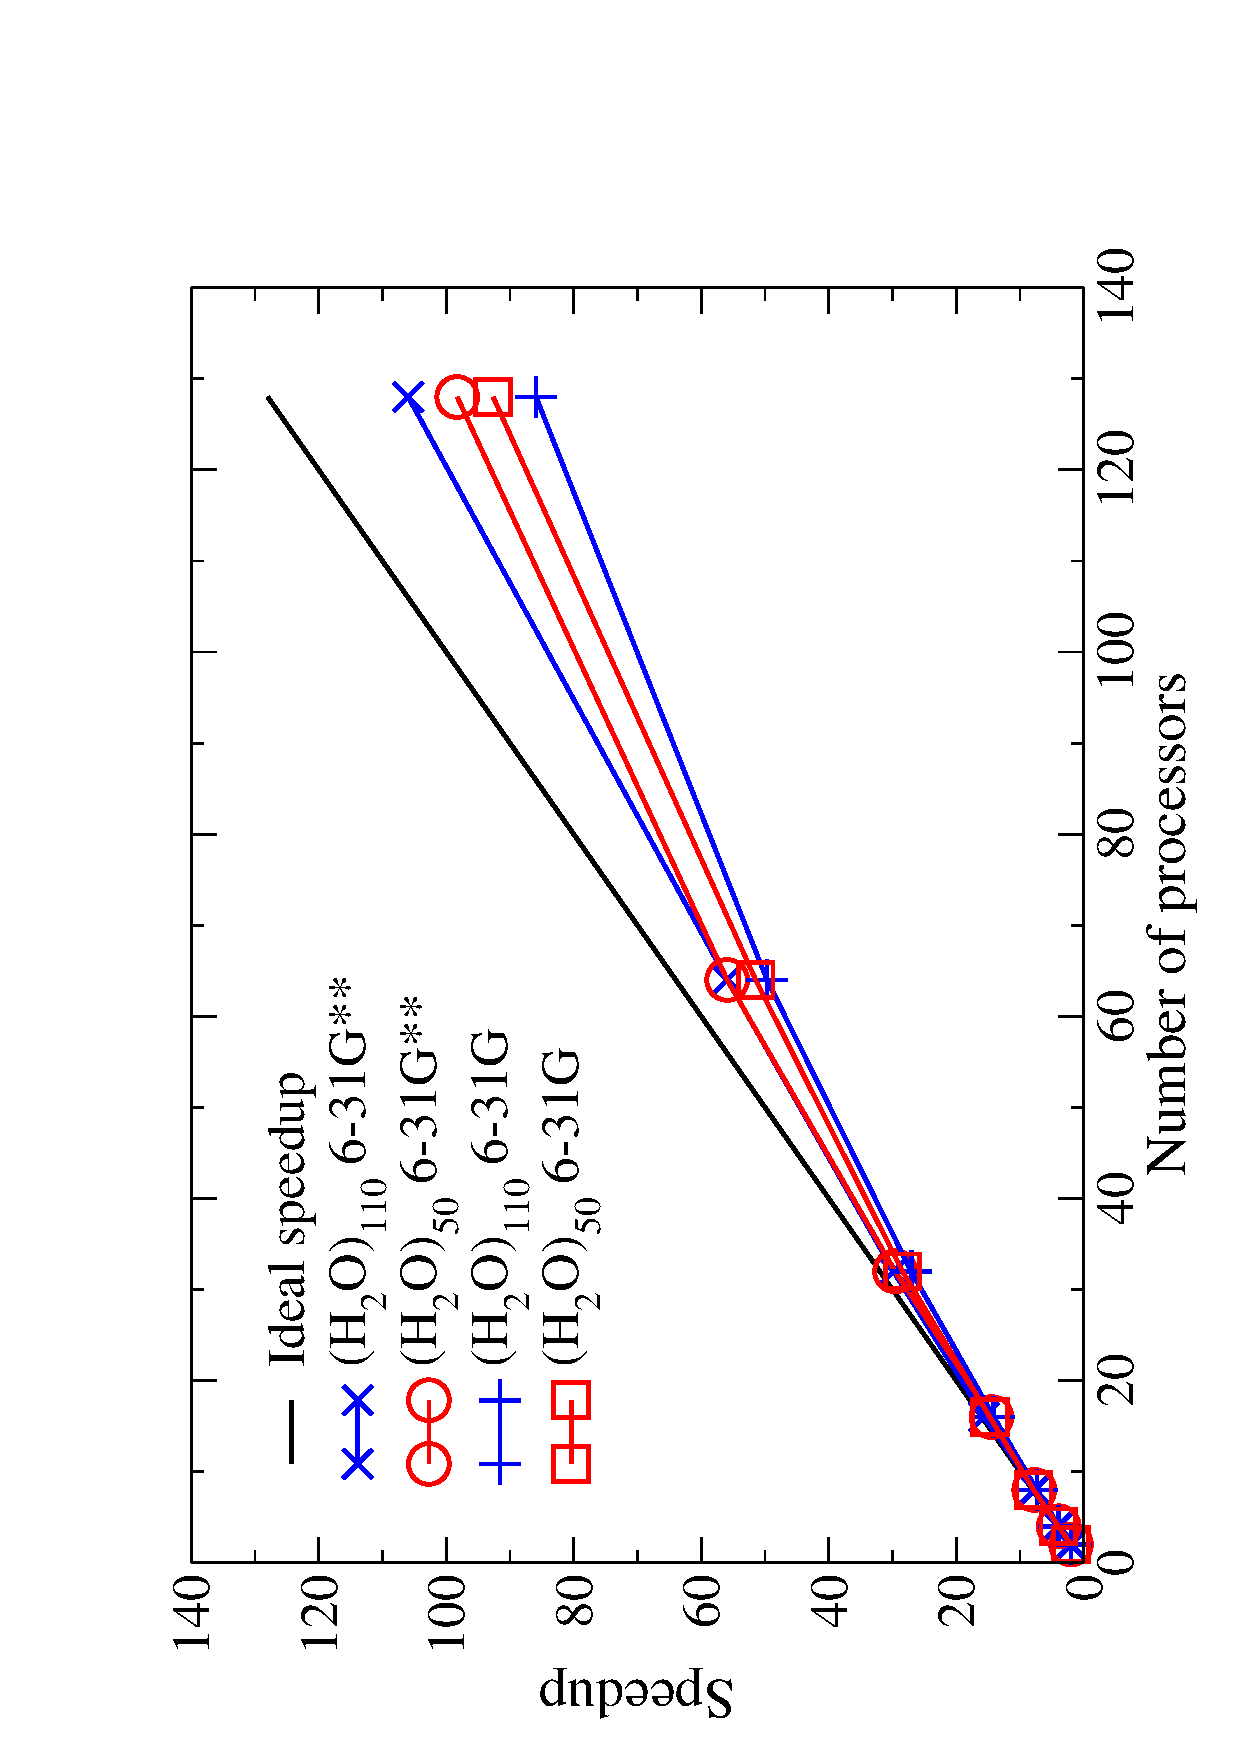
\includegraphics[angle=-90,width=0.5\textwidth]{h2o_50_110}
\end{figure}


\begin{figure}[h]
  \caption{\protect
    Relative speedup of the parallel ONX on (H$_2$O)$_{50}$ with the RHF/6-31G**
    along the SCF iterations.
    Speedups are relative to 2 processors.
  }\label{fig:h2o_50_prop}
  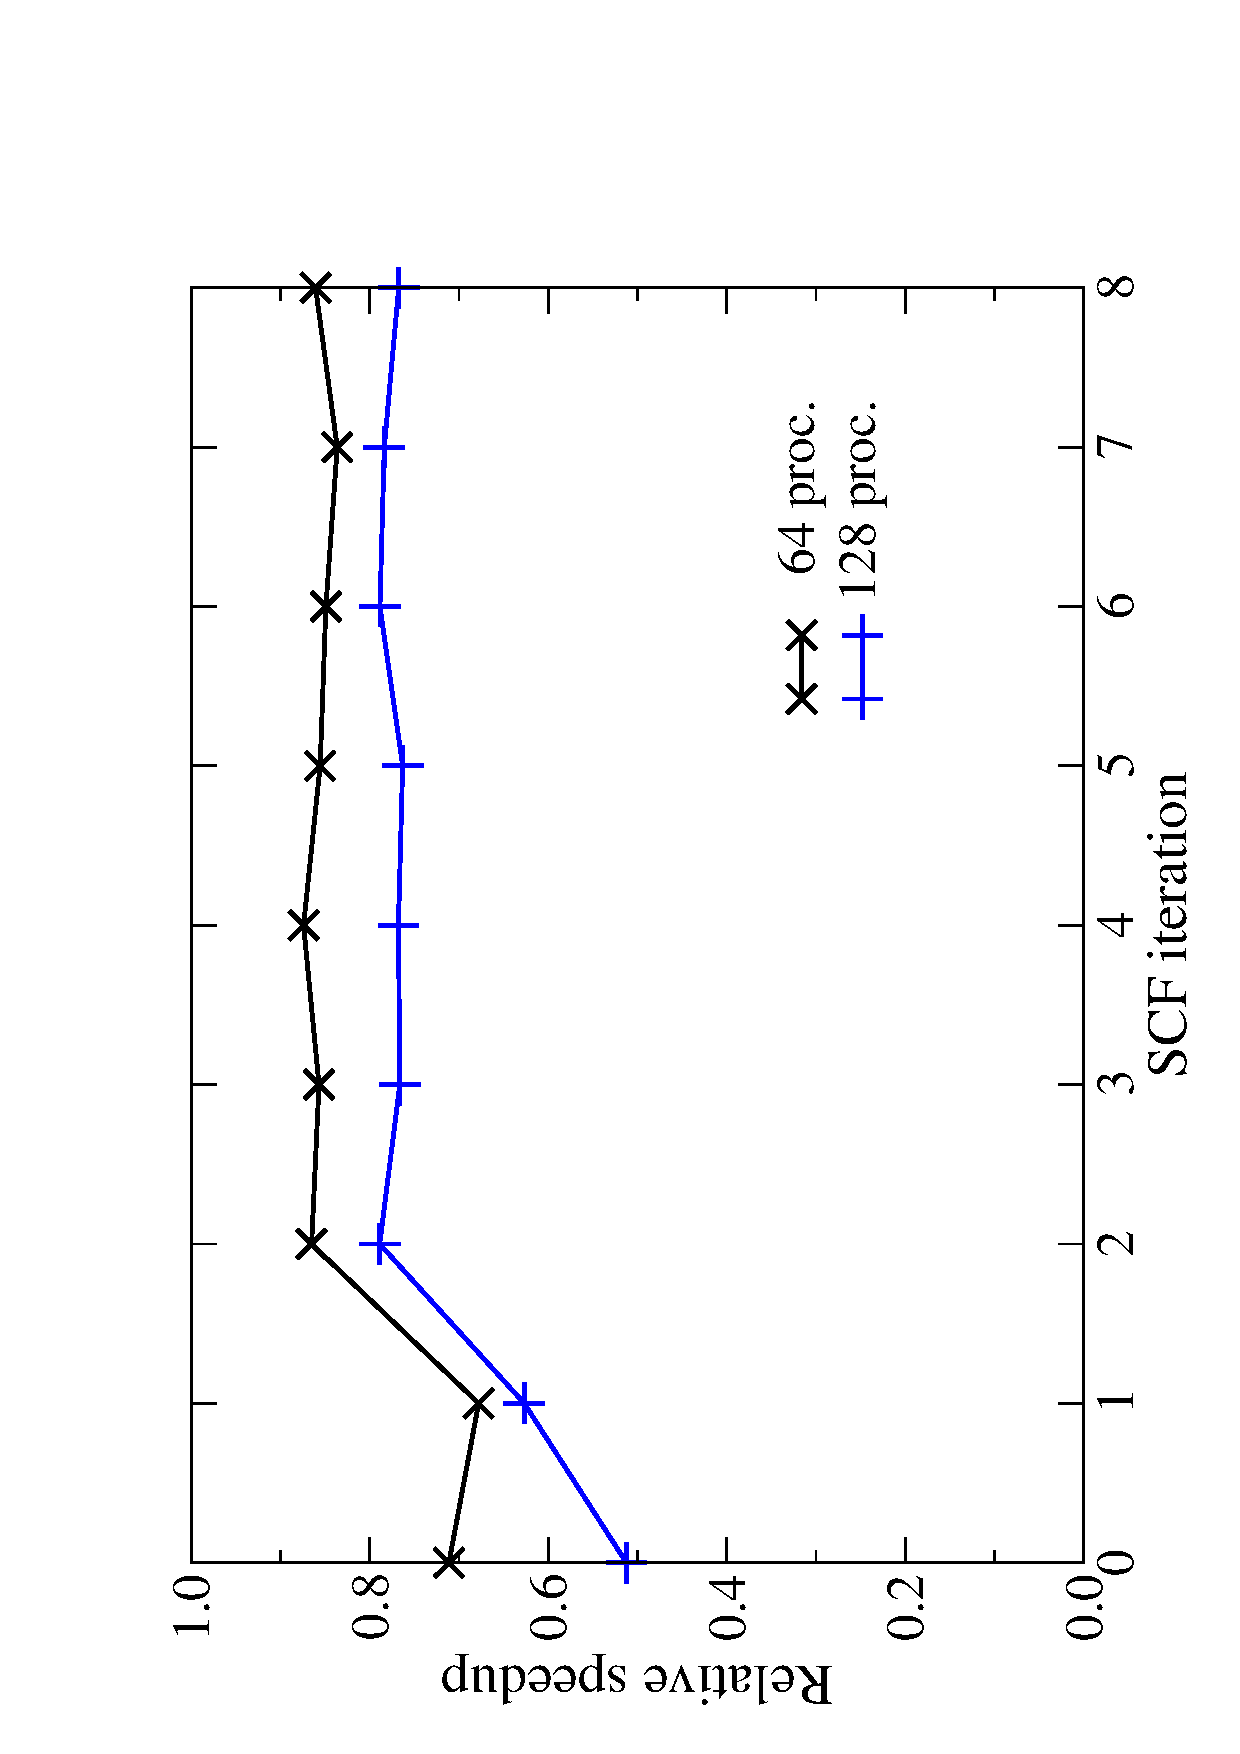
\includegraphics[angle=-90,width=0.5\textwidth]{h2o_50_prop}
\end{figure}

\subsection{Water box with PBC}
 For the periodic systems, the result of the 64-water molecules obtained on the BProc cluster is shown
 in Fig.~\ref{fig:h2o_pbc_64}. The calculations are performed at the
 RHF level of theory with the 6-31G*(O)/5-11G*(H), 6-31G and 6-31G** basis sets and the {\tt GOOD} accuracy. 
% An efficiency of $87\%$ is observed with 128 processors, which corresponds to
% a speedup of about $112$. 
 Efficiencies are $87\%$, $75\%$ and $79\%$ for the 6-31G*/5-11G*, 6-31G and 6-31G** 
 basis sets respectively, with 128 processors. The overall parallel ONX is very
 good up to 64 processors but degrades slightly at the 128-processor level.

 These performances, obtained for the water box, are better compared to the (H$_2$O)$_{50}$ cluster. The 
 improved speedup is due to the longer time spent in the
 exchange build for the periodic cases compared 
 to the gas phase cases. As the computation time spent in the innermost loop 
 increases, due to the double summations over lattice vectors,
 the timing function gives a more accurate elapsed time for each 
 atom-block of the density matrix.\\

\begin{figure}[p]
  \caption{\protect
    Scaling of the parallel ONX on (H$_2$O)$_{64}$ PBC with the RHF/6-31G*(O)/5-11G*(H),
    the RHF/6-31G** and RHF/6-31G level of theories and the {\tt GOOD} threshold. 
    The speedups are relative to 2 processors.
  }\label{fig:h2o_pbc_64}
  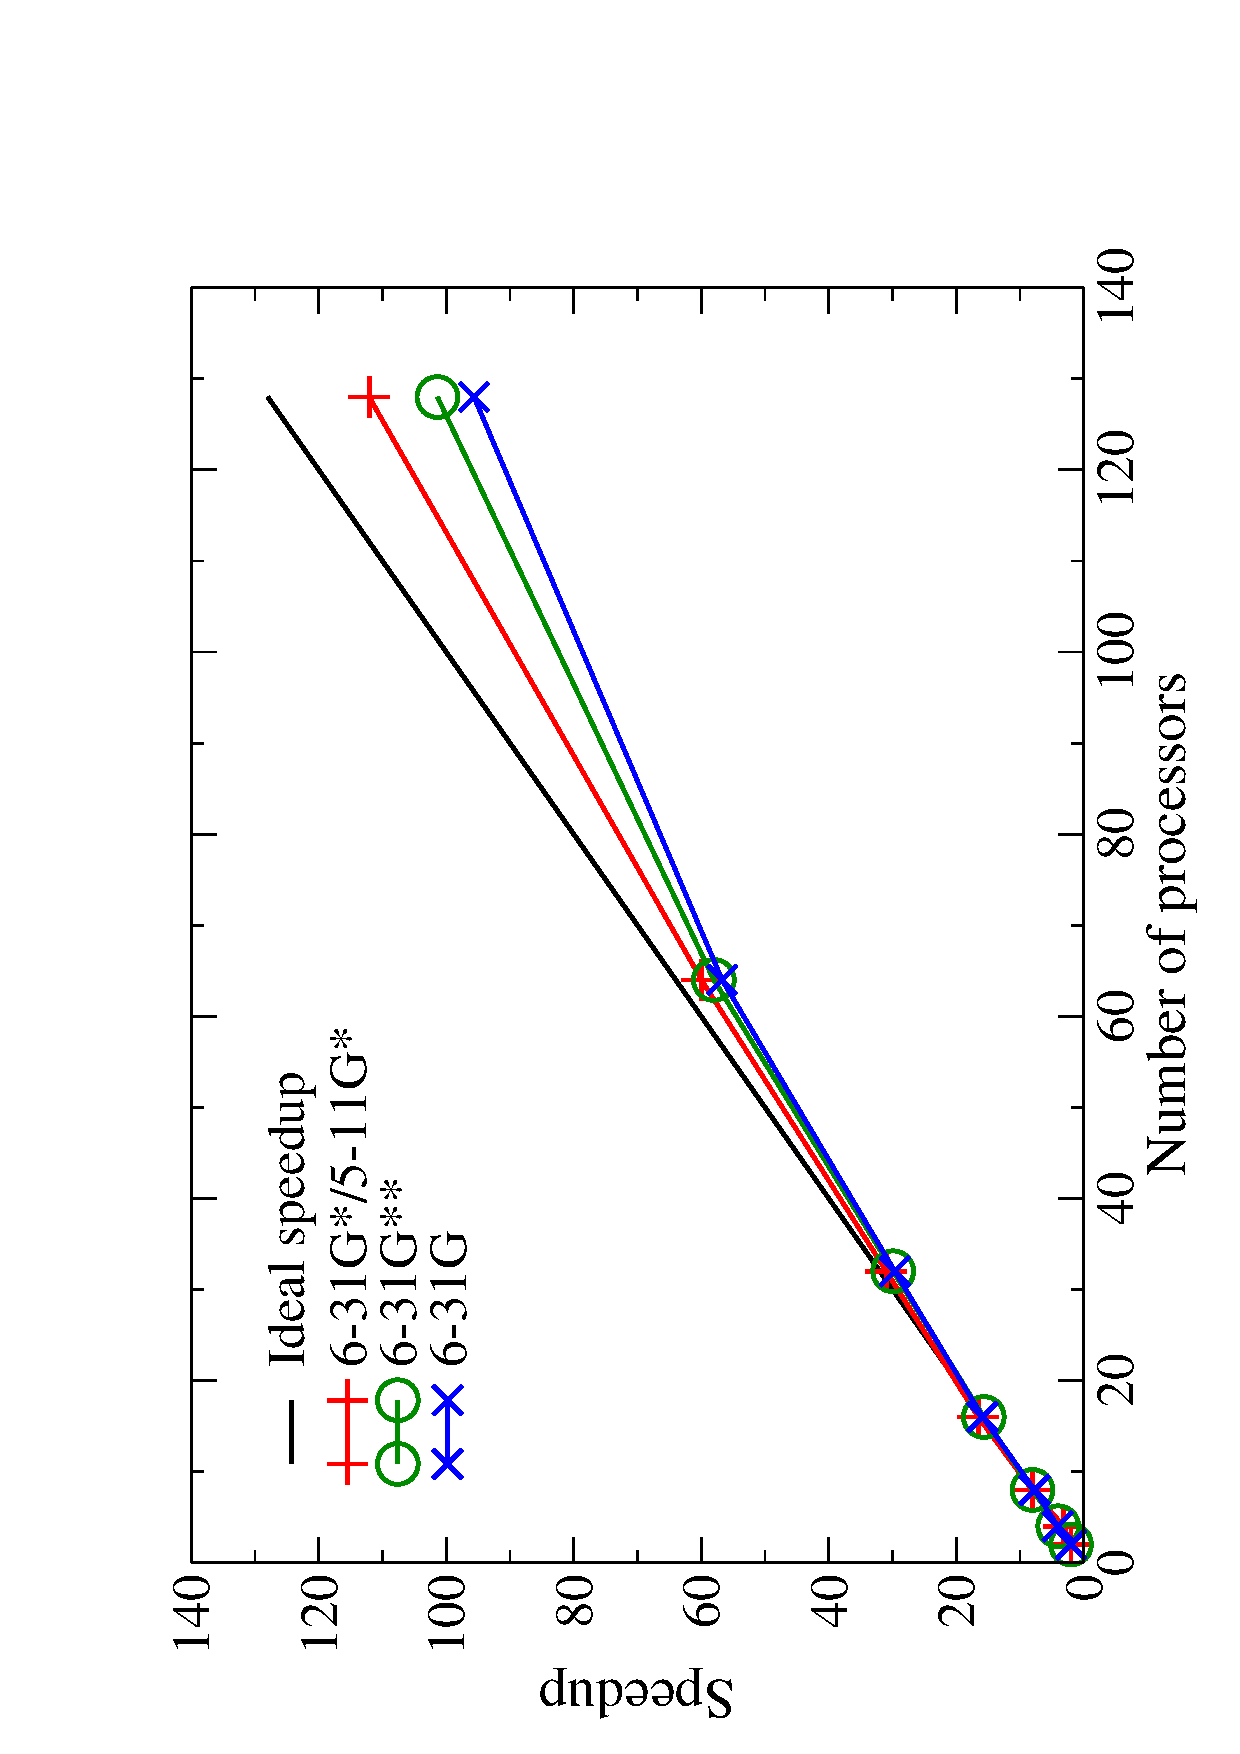
\includegraphics[angle=-90,width=0.5\textwidth]{h2o_pbc_64}
\end{figure}

\subsection{Endothelin and periodic KCNS}
Finally, we present, in Fig.~\ref{fig:Endothelin_KCNS}, 
speedup obtained on the Compaq machine for 
endothelin (C$_{82}$H$_{122}$O$_{26}$N$_{20}$S$_5$) and
for a orthorhombic supercell composed of 32 KCNS ($P_{bcm}$)
at the RHF/6-31G** and RHF/86-511G(K)/86-311G(S)/6-311G(C,N) 
level of theories, respectively.
These scaling have been carried out with the {\tt GOOD} accuracy level.
At the 128-processor level, the endothelin (133 heavy atoms) delivers 99 fold
speedup, while the $2\times 2\times 2$ KCNS (128 atoms per simulation supercell)
delivers 105 fold speedup. 
We also show in Fig.~\ref{fig:EndothelinTotalTiming} the total speedup 
of the fourth SCF for endothelin as well as the three most consuming parts of the SCF
{\em i.e.} the Coulomb build (Quantum Chemical Tree Code QCTC~\cite{MChallacombe97}),
the exact exchange build (ONX) and the density matrix solver (TRS4).

\begin{figure}[p]
  \caption{\protect
    Scaling of the parallel ONX on Endothelin and periodic (KCNS)$_{32}$ with 
    the RHF/6-31G** and RHF/86-511G(K)/86-311G(S)/6-311G(C,N) 
    respectively and the {\tt GOOD} threshold.
    The speedups are relative to 2 processors.
  }\label{fig:Endothelin_KCNS}
  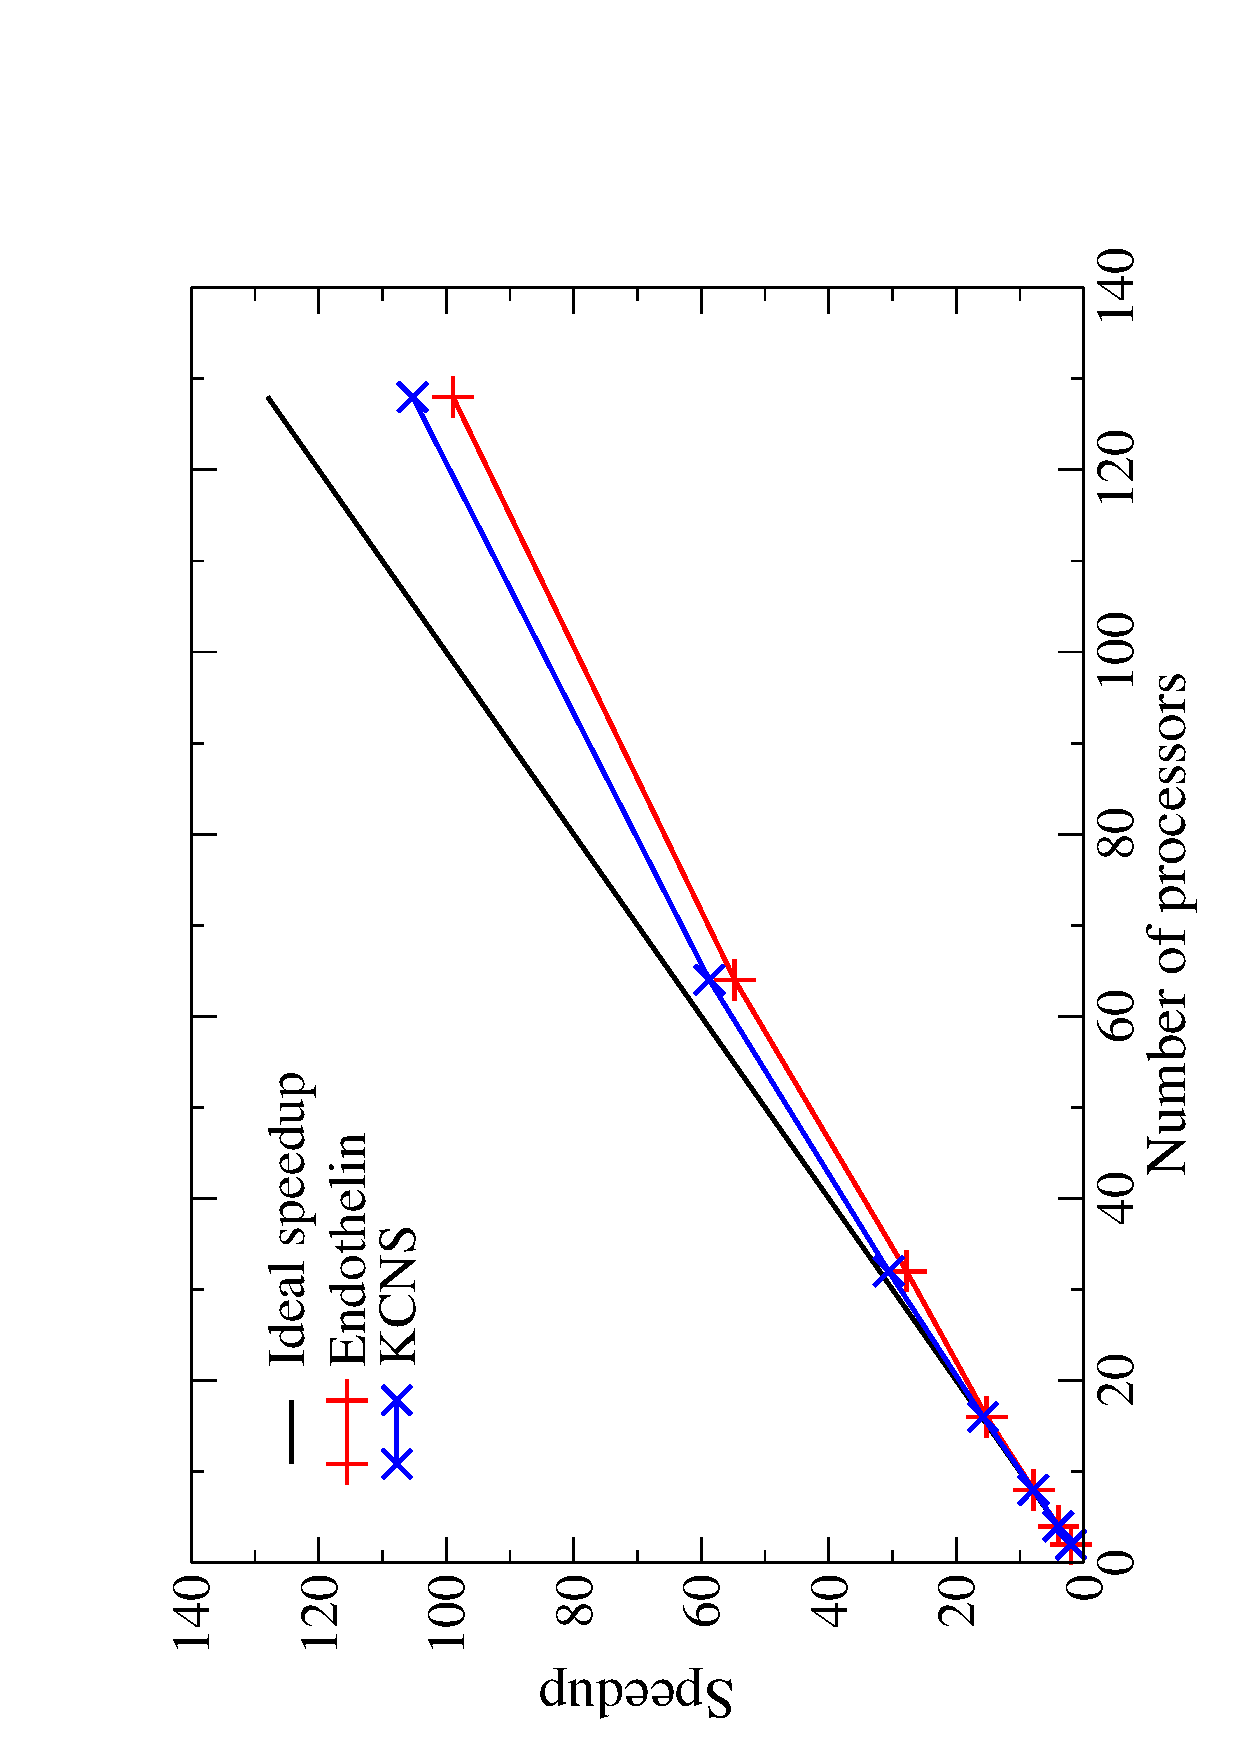
\includegraphics[angle=-90,width=0.5\textwidth]{Endothelin_KCNS}
\end{figure}

\begin{figure}[p]
  \caption{\protect
    Total scaling of the parallel SCF and its most consuming parts 
    on Endothelin with the RHF/6-31G**  
    and the {\tt GOOD} threshold. 
    The speedups are relative to 2 processors.
  }\label{fig:EndothelinTotalTiming}
  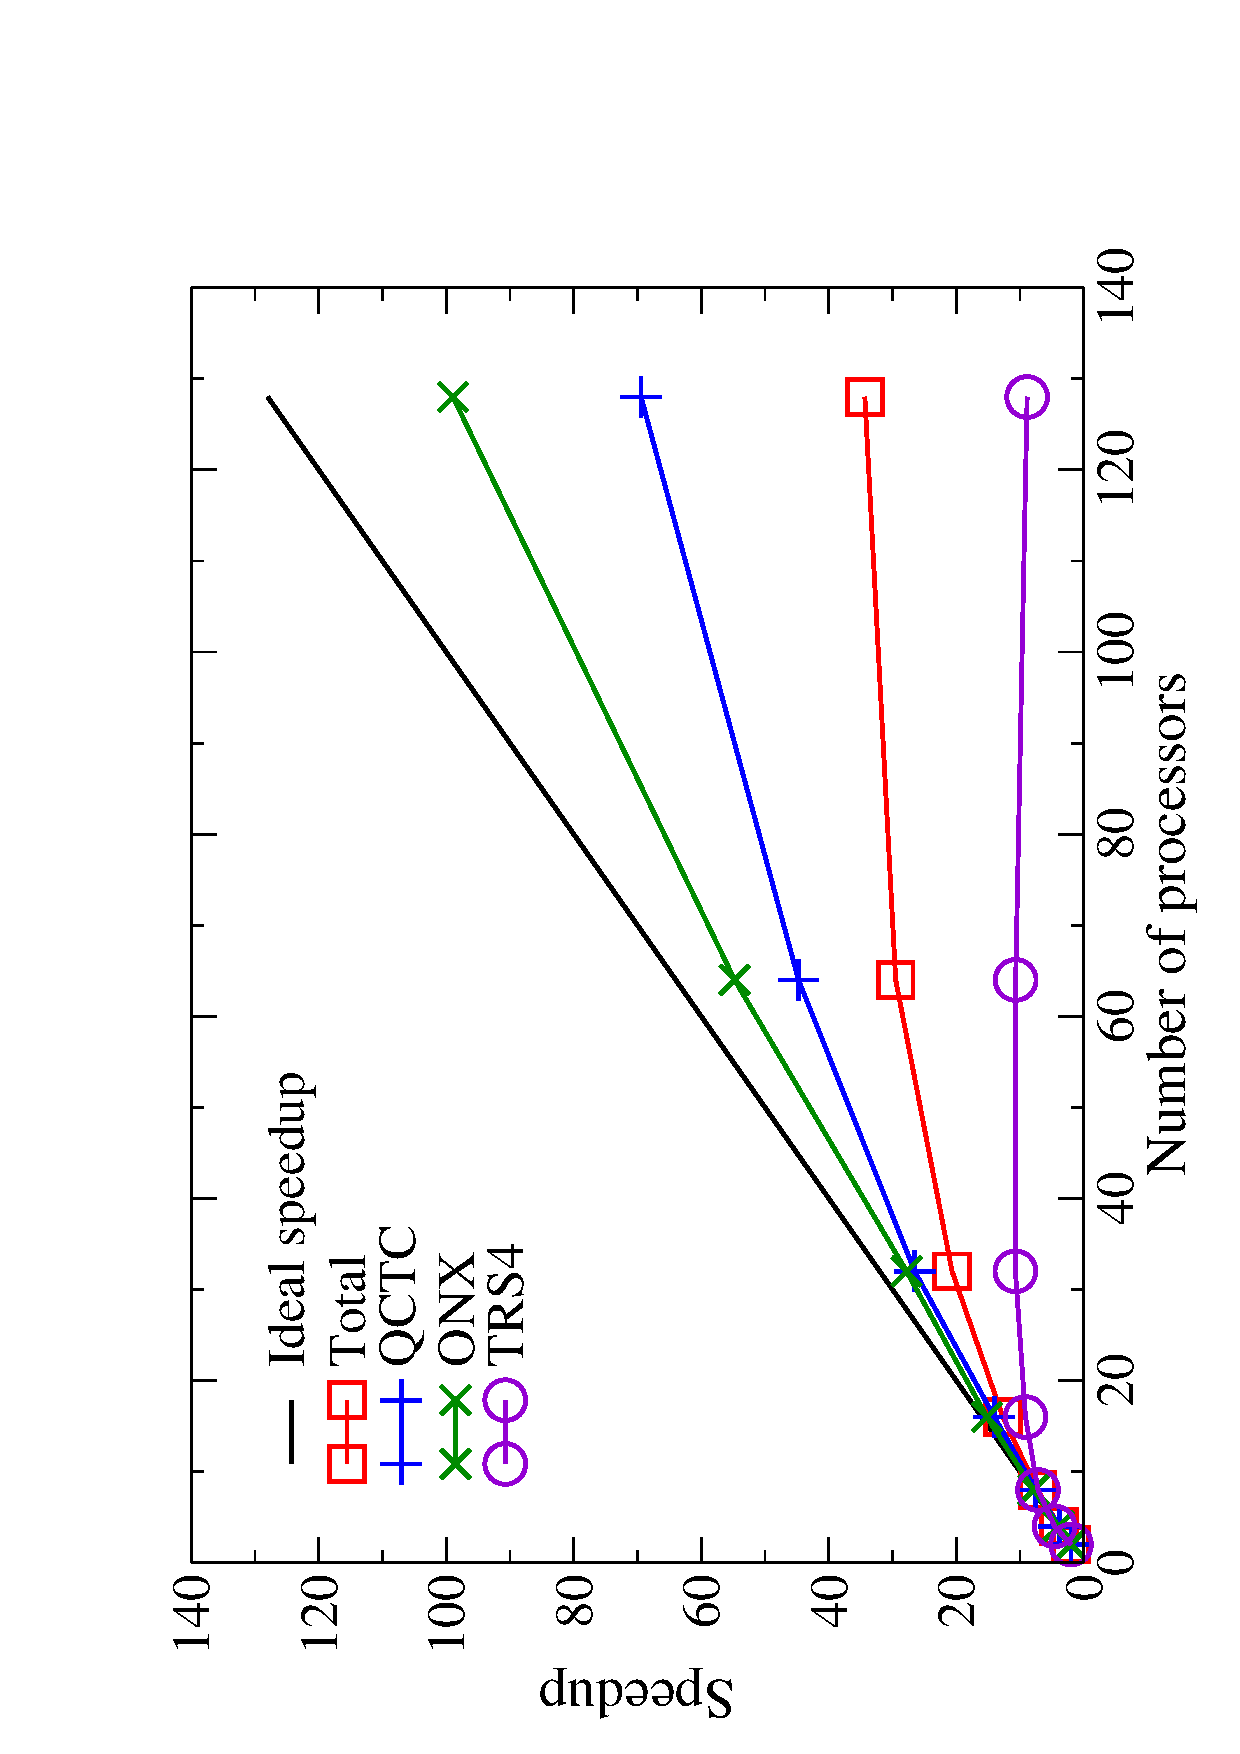
\includegraphics[angle=-90,width=0.5\textwidth]{EndothelinTotalTiming}
\end{figure}

%%%%%%%%%%%%%%%%%%%%%%%%%%%%%%%%%%%%%%%%%%%%%%%%%%%%%%%%%%%%%%%%
%%%%%%%%%%%%%%%%%%%%%%%%%%%%%%%%%%%%%%%%%%%%%%%%%%%%%%%%%%%%%%%%
\section{Conclusion}\label{Sec:Conc}

 We have presented a simple and efficient algorithm for 
 parallelization of the exact Hartree-Fock
 exchange. The method is based on the dynamical distribution 
 of the density matrix to the processors. At each SCF cycle the
 time needed to build the local exchange matrix corresponding
 to the local density matrix on a given processor is used to
 distribute the density matrix in the next cycle. 

 The concept of ET has proven fruitful for load balancing the ONX 
 algorithm. ET exploits the ``slow'' variation of the density matrix 
 between SCF iterations to overcome the irregularities arising 
 from the ${\cal O}(N)$ methods.

 A finer grain partition of the density matrix ({\em i.e.} at the function level)
 may lead to even better load balance. However, the code 
 may become much slower due to the non-negligible overhead 
 of the timing routine.

 The overall efficiency of the ET partition ranges from 74-87\%
 for all test cases presented in this work with the fine grained
 (up to 2.56 processors per heavy atom) 128 processor calculations.
 This high efficiency of the ET retains this property between geometry steps
 in a geometry optimization or molecular dynamics run after
 few steps (usually less than 3) of stabilization of the density matrix.

 We can also note that the ONX algorithm includes non-parallel step as
 loading, distributing the density matrix to all
 processors, global summation and I/O. Thus we may expect 
 the efficiency to improve with full data parallelism.

% Total timing for the parallel SCF including Fock build, 
% density matrix solver, convergence acceleration method and I/O will be addressed in a 
% forthcoming paper~\cite{MONDOParallelSCF}.

%%%%%%%%%%%%%%%%%%%%%%%%%%%%%%%%%%%%%%%%%%%%%%%%%%%%%%%%%%%%%%%%
%%%%%%%%%%%%%%%%%%%%%%%%%%%%%%%%%%%%%%%%%%%%%%%%%%%%%%%%%%%%%%%%
\begin{acknowledgments}
 This work has been supported by the US Department of Energy
 under contract W-7405-ENG-36 and the ASCI project.
 The Advanced Computing Laboratory of Los
 Alamos National Laboratory is acknowledged.
\end{acknowledgments}
%%%%%%%%%%%%%%%%%%%%%%%%%%%%%%%%%%%%%%%%%%%%%%%%%%%%%%%%%%%%%%%%
%%%%%%%%%%%%%%%%%%%%%%%%%%%%%%%%%%%%%%%%%%%%%%%%%%%%%%%%%%%%%%%%
\bibliography{mondo_new}
%\bibliography{pONX,mondo_new}
\newpage
%%%%%%%%%%%%%%%%%%%%%%%%%%%%%%%%%%%%%%%%%%%%%%%%%%%%%%%%%%%%%%%%
%%%%%%%%%%%%%%%%%%%%%%%%%%%%%%%%%%%%%%%%%%%%%%%%%%%%%%%%%%%%%%%%


\commentoutB{


\clearpage

\begin{center}
\bf  TABLES\\[1.cm]
\end{center}

\clearpage

\begin{figure}[h]
\begin{center}
\bf  FIGURES\\[1.cm]
\end{center}

%\caption{\protect  Total CPU time of the fifth CPSCF iteration for the water cluster sequence with
%         the 6-31G and 6-31G** basis sets and the {\tt GOOD} and {\tt TIGHT} numerical thresholds (see text)
%         controlling numerical precision of the result.  The lines are fits to the last three and four points, respectively.}\label{scaling}

\end{figure}

\clearpage

\begin{center}
Figure 1, V.~Weber and M.~Challacombe \\[1.cm]
%\resizebox*{5in}{!}{\includegraphics{figure1.eps}}
\end{center}

\clearpage

\begin{center}
Figure 2, V.~Weber  and M.~Challacombe \\[1.cm]
%\resizebox*{7in}{!}{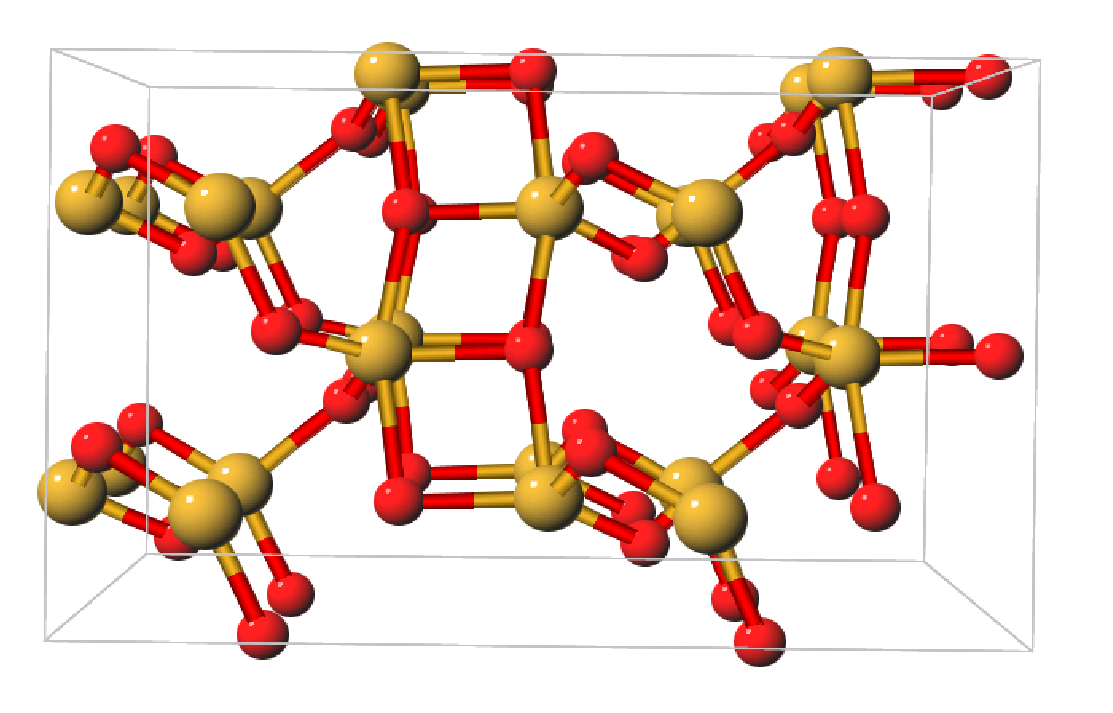
\includegraphics{figure2.eps}}
\end{center}

\clearpage

\begin{center}
Figure 3, V.~Weber  and M.~Challacombe \\[1.cm]
%\resizebox*{7in}{!}{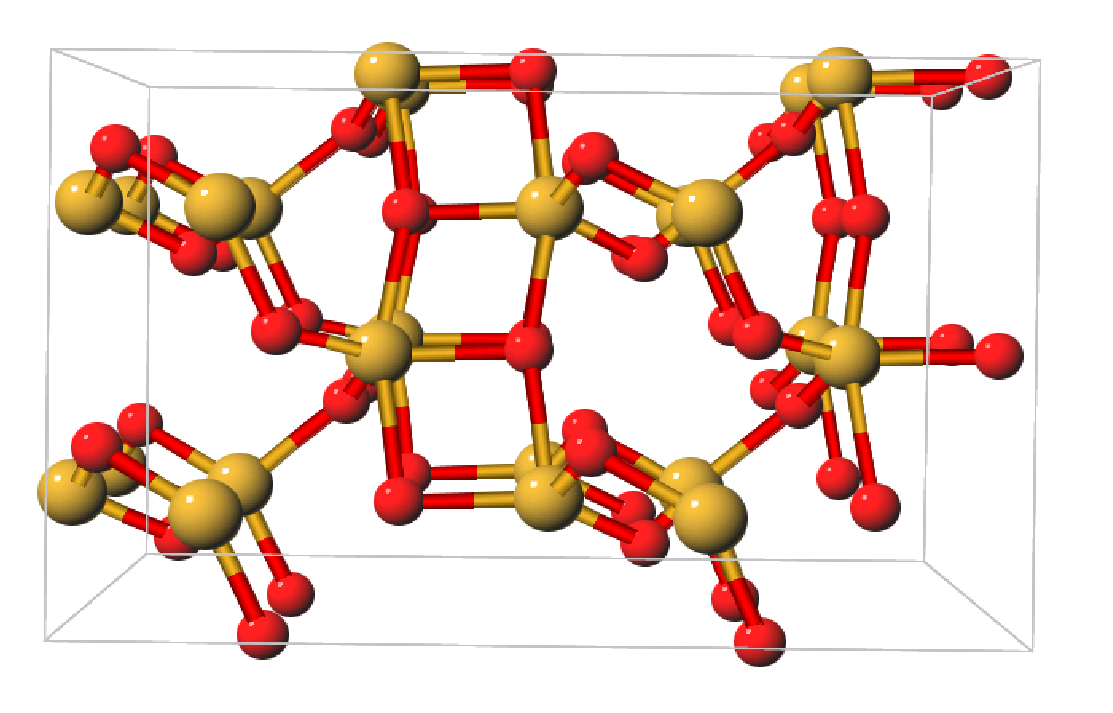
\includegraphics{figure2.eps}}
\end{center}

\clearpage

\begin{center}
Figure 4, V.~Weber  and M.~Challacombe \\[1.cm]
%\resizebox*{7in}{!}{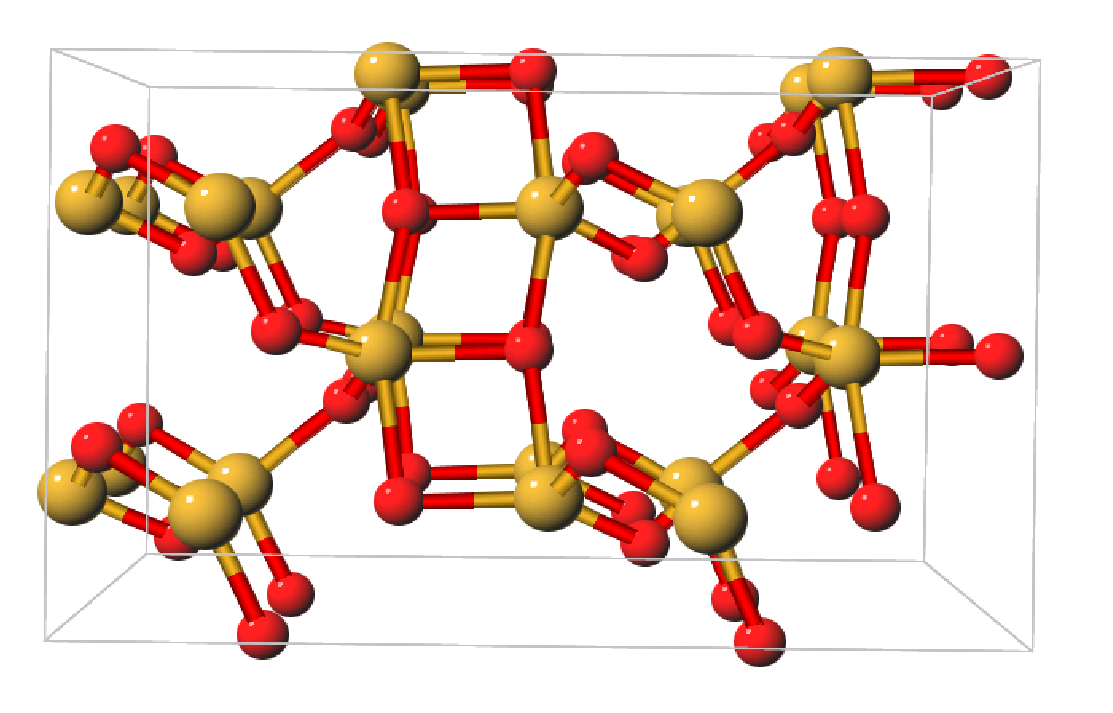
\includegraphics{figure2.eps}}
\end{center}

\clearpage

\begin{center}
Figure 6, V.~Weber  and M.~Challacombe \\[1.cm]
%\resizebox*{7in}{!}{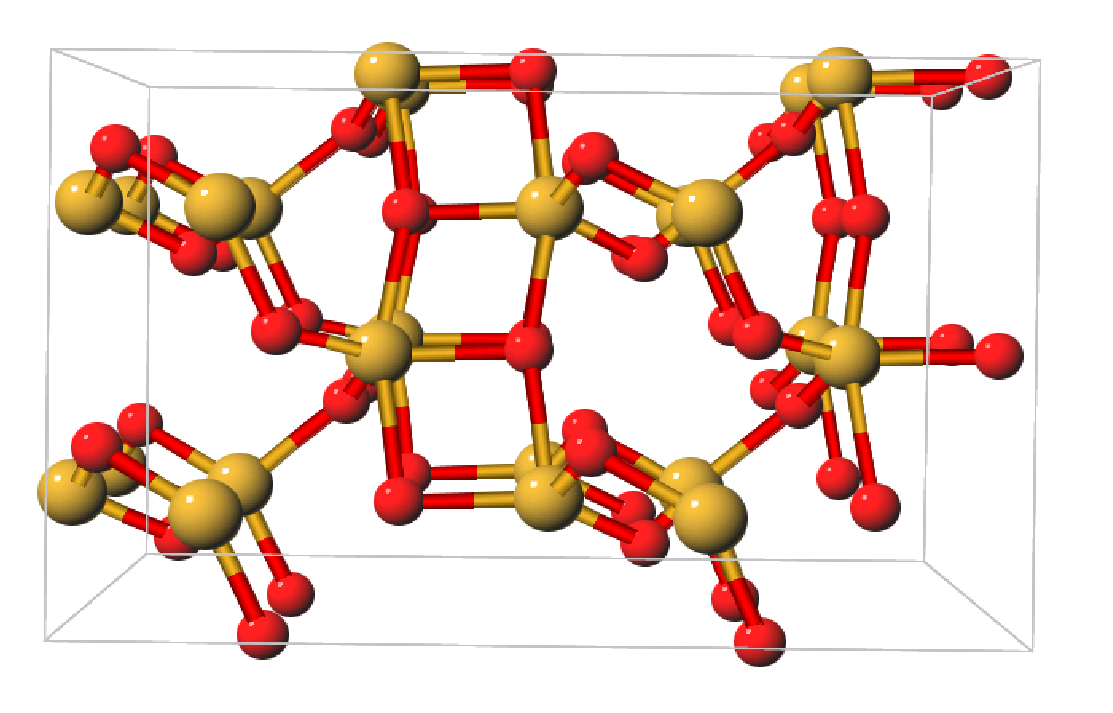
\includegraphics{figure2.eps}}
\end{center}

\clearpage

\begin{center}
Figure 7, V.~Weber  and M.~Challacombe \\[1.cm]
%\resizebox*{7in}{!}{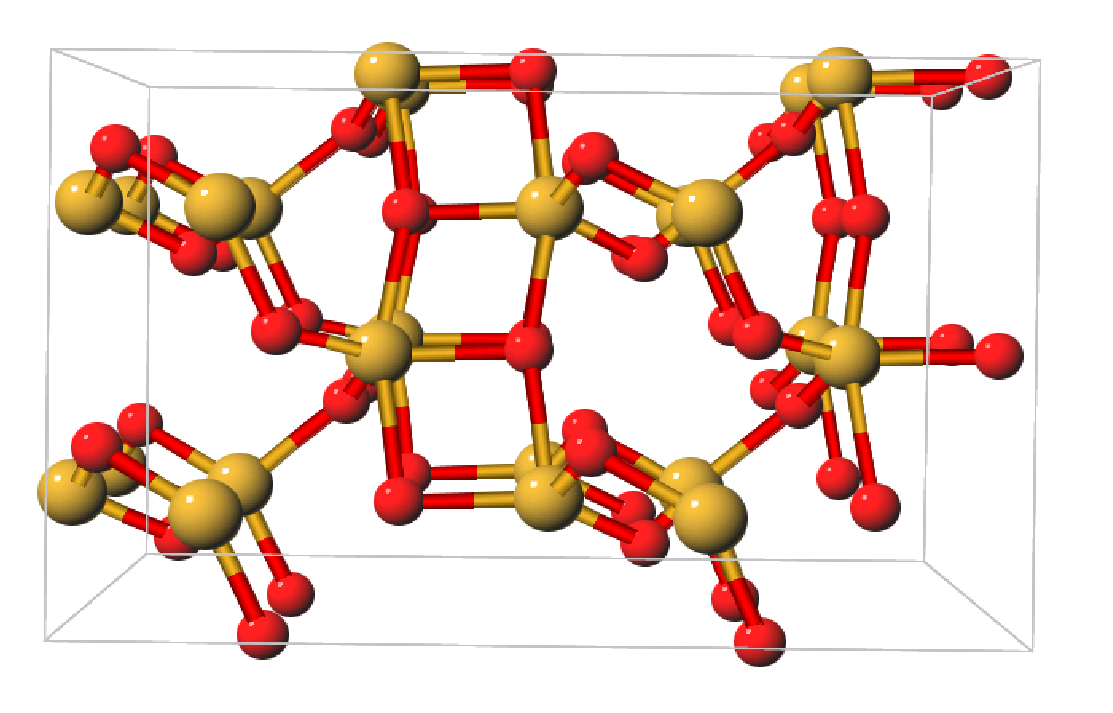
\includegraphics{figure2.eps}}
\end{center}

\clearpage

\begin{center}
Figure 8, V.~Weber  and M.~Challacombe \\[1.cm]
%\resizebox*{7in}{!}{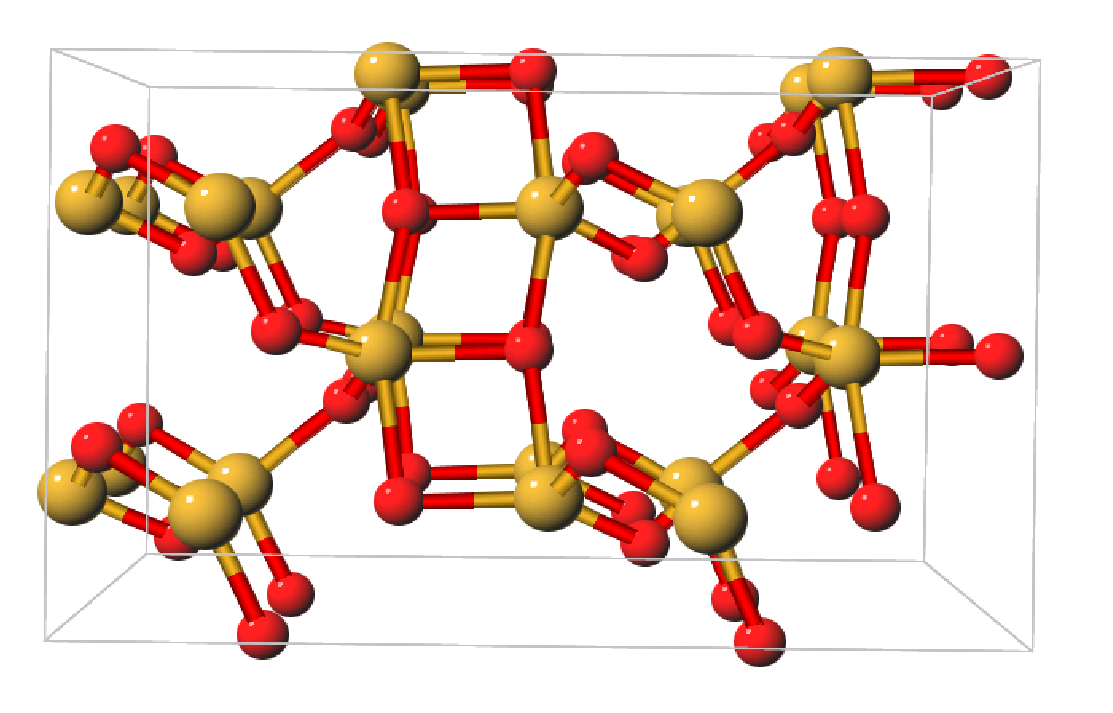
\includegraphics{figure2.eps}}
\end{center}



} %commentoutB

%%%%%%%%%%%%%%%%%%%%%%%%%%%%%%%%%%%%%%%%%%%%%%%%%%%%%%%%%%%%%%%%
%%%%%%%%%%%%%%%%%%%%%%%%%%%%%%%%%%%%%%%%%%%%%%%%%%%%%%%%%%%%%%%%
%%%%%%%%%%%%%%%%%%%%%%%%%%%%%%%%%%%%%%%%%%%%%%%%%%%%%%%%%%%%%%%%
\end{document}
%
% ****** End of file apssamp.tex ******

